\documentclass[tikz,border=0pt]{standalone}
\usepackage[compat=1.1.8]{tikz-feynman}
\usepackage{amsmath}
\usetikzlibrary{calc,positioning,shadows.blur,decorations.pathreplacing}





%% particles
\newcommand{\PZ}{\ensuremath{\text{Z}}}
\newcommand{\PH}{\ensuremath{\text{H}}}
\newcommand{\PW}{\ensuremath{\text{W}}}
\newcommand{\PWp}{\ensuremath{\text{W}^{+}}}
\newcommand{\PWm}{\ensuremath{\text{W}^{-}}}
\newcommand{\PWpm}{\ensuremath{\text{W}^{\pm}}}
\newcommand{\PJPsi}{\ensuremath{\text{J}/\Psi}}
\newcommand{\PPsiPrime}{\ensuremath{\Psi^{\prime}}}
\newcommand{\PPsiS}{\ensuremath{\Psi(\text{1S})}}
\newcommand{\PPsiSS}{\ensuremath{\Psi(\text{2S})}}
\newcommand{\PPsiNS}{\ensuremath{\Psi(\text{nS})}}





\begin{document}
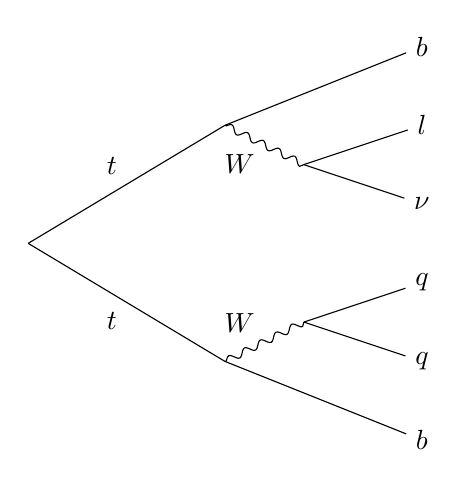
\begin{tikzpicture}
  \begin{feynman}
    \vertex (a) at (0,0) ;
    \vertex [] at (2.5,1.5) (t1);
    \vertex [] at (2.5,-1.5) (t2);
    \vertex [] at (5,2.5) (b1) {\(b\)};
    \vertex [] at (3.5,1) (w1);
    \vertex [] at (5,1.5) (l1) {\(l\)};
    \vertex [] at (5,0.5) (v1) {\(\nu\)};
    \vertex [] at (3.5,-1) (w2);
    \vertex [] at (5,-0.5) (q1) {\(q\)};
    \vertex [] at (5,-1.5) (q2) {\(q\)};
    \vertex [] at (5,-2.5) (b2) {\(b\)};

    \diagram* {
      (a) -- [edge label=\(t\)] (t1),
      (a) -- [edge label'=\(t\)] (t2),
      (t1) -- [] (b1),
      (t1) -- [boson, edge label'=\(W\)] (w1),
      (w1) -- [] (l1),
      (w1) -- [] (v1),
      (t2) -- [boson, edge label=\(W\)] (w2),
      (w2) -- [] (q1),
      (w2) -- [] (q2),
      (t2) -- [] (b2)
    };
  \end{feynman}
\end{tikzpicture}
\end{document}